%================================================================
\chapter{Adversarial Self-Play}
\label{ch:selfplay}
%================================================================

\section{Motivation}
\label{sec:selfplay_motivation}

The Temporal \moe{} defender trained in Chapter~\ref{ch:architecture}
was evaluated against a fixed set of hand-crafted attacks. A defender
that performs well on a fixed attack distribution does not necessarily
perform well against an attacker who adapts. In a real deployment,
an adversary who knows or can approximate the defender model will
craft perturbations designed to evade it.

The standard answer is adversarial training: generate adversarial
examples and train the defender on them. The limitation is that the
adversarial example generator is fixed, so the training distribution
is fixed, and the defender learns to resist that specific generator.

Self-play removes this limitation by making the attacker itself a
learned model that co-evolves with the defender. When the defender
gets better at catching a particular attack strategy, the attacker's
loss increases and it is pushed towards new strategies. When the
attacker discovers a new strategy, the defender's loss increases and
it is updated to catch it. At convergence (or at the best validation
checkpoint), the defender has been trained against the space of
attacks that can be generated by a \gnn{}-parametrised attacker
within the stealth budget.

\section{Attacker Model}
\label{sec:attacker_model}

\subsection{Architecture}

The attacker, \texttt{AttackerGNN}, shares the GraphSAGE
backbone with the defender but replaces the prediction heads. The
backbone produces node embeddings $\mathbf{H} \in \mathbb{R}^{N \times d}$.
Four heads operate on these embeddings:

\begin{description}
  \item[Pressure delta head] $\hat{\delta}_p = \varepsilon \cdot
    \tanh(\mathrm{MLP}(\mathbf{H}))$, outputting a perturbation in
    $(-\varepsilon, +\varepsilon)$ for each node. The $\tanh$
    squashing means the stealth budget projection needs only
    to zero out low-ranked sensors.
  \item[Pressure mask head] $\hat{m}_p = \mathrm{MLP}(\mathbf{H})$,
    outputting logits for ``attack this sensor''.
  \item[Flow delta head] $\hat{\delta}_q = \varepsilon_q \cdot
    \tanh(\mathrm{MLP}([\mathbf{h}_i \| \mathbf{h}_j \| \mathbf{e}_{ij}]))$,
    outputting a perturbation per edge.
  \item[Flow mask head] $\hat{m}_q = \mathrm{MLP}([\mathbf{h}_i \|
    \mathbf{h}_j \| \mathbf{e}_{ij}])$.
\end{description}

\subsection{Stealth Budget Projection}
\label{sec:budget}

The raw attacker output is projected onto the feasible set defined
by the $(\varepsilon, k)$ budget as follows:

\begin{enumerate}
  \item Compute pressure mask probabilities
    $\mathbf{p}_m = \sigma(\hat{m}_p)$.
  \item Select the top-$k_p$ sensors by mask probability.
  \item For the selected sensors, apply
    $\tilde{p}_i = p_i^* + \hat{\delta}_{p,i}$.
  \item For all others, $\tilde{p}_i = p_i^*$ (no perturbation).
\end{enumerate}
The same procedure applies to flow sensors with budget $(k_q,
\varepsilon_q)$.

This projection is differentiable with respect to the mask
logits (via the straight-through estimator for the top-$k$
selection) and with respect to the delta values (direct gradient).
In practice the gradient through the top-$k$ selection is noisy but
sufficient for training.

\subsection{Physics Penalty}

The attacker's perturbation may violate mass conservation at attacked
nodes. A physics penalty penalises this:
\begin{equation}
  \mathcal{L}_\text{physics} = \frac{\lambda_\text{phys}}{N}
    \left\|\mathbf{B}(\hat{\mathbf{q}} + \hat{\boldsymbol{\delta}}_q)
    - \mathbf{d}\right\|_2^2.
\end{equation}
Setting $\lambda_\text{phys} = 0.05$ in the headline run means the
attacker is nudged towards physically plausible perturbations but
is not forced to satisfy conservation exactly. An attacker that
respects physics is harder to detect by hydraulic-model-based
detectors, which in practice are co-deployed with learned detectors
in real SCADA systems.

\section{Stackelberg Self-Play Loop}
\label{sec:stackelberg_loop}

\subsection{Alternating Optimisation}

The training loop alternates between attacker and defender updates.
In each epoch:

\begin{algorithm}[htbp]
  \DontPrintSemicolon
  \caption{Stackelberg Self-Play Training Loop}
  \label{alg:selfplay}
  \KwIn{Pretrained defender $f_\theta$; empty attacker $g_\phi$;
    budget $(\varepsilon, k)$; steps $S_a$, $S_d$}
  \For{each epoch}{
    \tcc{Attacker update phase (defender frozen)}
    Freeze $f_\theta$\;
    \For{$s = 1, \ldots, S_a$}{
      Sample mini-batch of windows\;
      $\tilde{\mathbf{x}} \leftarrow \text{ApplyBudget}(g_\phi(\mathbf{x}),
        \varepsilon, k)$\;
      $\hat{\mathbf{y}} \leftarrow f_\theta(\tilde{\mathbf{x}})$\;
      $\mathcal{L}_\text{atk} = -\lambda_\text{recon}
        \mathcal{L}_\text{damage} + \mathcal{L}_\text{stealth}
        + \lambda_\text{phys}\mathcal{L}_\text{physics}$\;
      Update $\phi$ via Adam\;
    }
    \tcc{Defender update phase (attacker frozen)}
    Unfreeze $f_\theta$; freeze $g_\phi$\;
    \For{$s = 1, \ldots, S_d$}{
      Sample mini-batch; generate $\tilde{\mathbf{x}}$ from $g_\phi$\;
      $\mathcal{L}_\text{def} = \mathcal{L}_\text{recon}
        + \lambda_\text{anomaly}\mathcal{L}_\text{anomaly}
        + \lambda_\text{router}\mathcal{L}_\text{router}$\;
      Update $\theta$ via Adam\;
    }
    \If{val F1 improves}{Save checkpoint\;}
  }
\end{algorithm}

The ratio $S_a : S_d = 3 : 1$ in the headline runs. More attacker
steps per defender step means the attacker has more opportunity to
explore new strategies before the defender adapts, producing a harder
training signal. The imbalance is empirically tuned; equal steps
lead to slower attacker convergence.

\subsection{Attacker Loss Components}

The attacker's loss has three terms:

\textbf{Damage loss} $\mathcal{L}_\text{damage}$: the reconstruction
MSE of the defender on the attacked sensors. Maximising
damage means the attacker produces perturbations that cause large
reconstruction errors. The negative sign in Algorithm~\ref{alg:selfplay}
means the attacker minimises negative damage, i.e., maximises it.

\textbf{Stealth loss} $\mathcal{L}_\text{stealth}$: the defender's
anomaly logit at attacked sensors, treated as a binary cross-entropy
with target 0 (``not anomalous''):
\begin{equation}
  \mathcal{L}_\text{stealth} = \frac{1}{|\mathcal{A}|}
    \sum_{i \in \mathcal{A}} \mathrm{BCE}(\hat{a}_i, 0),
\end{equation}
where $\mathcal{A}$ is the set of attacked sensors. The attacker
is rewarded for attacks that produce sensor readings the defender
rates as clean.

\textbf{Physics loss} $\mathcal{L}_\text{physics}$: continuity
violation penalty as in Section~\ref{sec:attacker_model}.

\subsection{Auto-Curriculum}
\label{sec:curriculum}

Starting with a tight budget $(\varepsilon_0, k_0)$ and gradually
relaxing it avoids mode collapse in the attacker: with too large a
budget from the start, the attacker trivially generates large
perturbations that are trivially detectable, and the defender
stagnates. The auto-curriculum monitors the validation adversarial
F1 and increases the budget when the defender is strong enough:

\begin{equation}
  \text{if } \mathrm{F1}_\text{val} > \tau_\text{curr},
  \text{ then }
  \varepsilon \leftarrow \min(\varepsilon + \Delta\varepsilon,
    \varepsilon_\text{max}),
  \quad
  k \leftarrow \min(k + \Delta k, k_\text{max}).
\end{equation}
In the headline Modena run:
$\varepsilon_0 = 3.0$\,m, $\varepsilon_\text{max} = 8.0$\,m,
$\Delta\varepsilon = 0.5$\,m, $k_0 = 10$, $k_\text{max} = 25$,
$\Delta k = 2$, $\tau_\text{curr} = 0.85$. The threshold fired
three times during the training run, ramping $k$ from 10 to 16.

\section{Mixture-of-Attackers}
\label{sec:attacker_moe}

\subsection{Motivation}

A single \texttt{AttackerGNN} converges to one attack strategy once
the defender can resist it. The defender then faces a training
distribution of measure one and over-fits to that single strategy.
An attacker \moe{} maintains a population of attackers with diverse
strategies, producing a richer training distribution for the defender.

\subsection{Architecture}

\texttt{MixtureOfAttackersGNN} wraps $K_\text{atk} = 4$ specialist
attackers and a shared router. The router, \texttt{AttackerRouter},
is a graph-pooling \gnn{} that produces a single vector per graph
and classifies it into one of the $K_\text{atk}$ experts. Per
snapshot, the router selects one expert (hard routing during
training, soft during evaluation) and that expert produces the
perturbation.

\subsection{Diversity and Balance Losses}

Two losses prevent mode collapse in the attacker population:

\textbf{Diversity loss}: penalises high cosine similarity between
the perturbation vectors of different experts on the same input:
\begin{equation}
  \mathcal{L}_\text{div} = \frac{1}{\binom{K}{2}}
    \sum_{j < k} \frac{\hat{\boldsymbol{\delta}}^{(j)} \cdot
      \hat{\boldsymbol{\delta}}^{(k)}}
      {\|\hat{\boldsymbol{\delta}}^{(j)}\|_2
       \|\hat{\boldsymbol{\delta}}^{(k)}\|_2}.
\end{equation}
Minimising this term pushes the experts towards orthogonal attack
strategies in perturbation space.

\textbf{Balance loss}: negative entropy of the batch-mean routing
probabilities, identical in form to Equation~\ref{eq:balance_loss}
for the defender.

The full attacker loss becomes:
\begin{equation}
  \mathcal{L}_\text{atk}^\text{MoE} =
    \mathcal{L}_\text{atk}^\text{single}
    + \lambda_\text{div}\mathcal{L}_\text{div}
    + \lambda_\text{bal}\mathcal{L}_\text{atk\text{-}balance}.
\end{equation}
Values $\lambda_\text{div} = 0.5$ and $\lambda_\text{bal} = 0.1$
are used in the headline run.

\subsection{Emergent Attack Vocabulary}

After training with no attack-class labels, the Attacker \moe{} uses
two of its four experts. Table~\ref{tab:vocab} summarises the
expert-class purity analysis from \texttt{vocabulary\_mining.py}: each
expert's perturbations are projected into 2D with t-SNE and
the ground-truth attack-class distribution within each expert's
assigned windows is tabulated.

\begin{table}[htbp]
  \centering
  \caption{Attack vocabulary discovered by the Attacker \moe{} on
  the Modena test set. Experts 0 and 1 receive fewer than 10
  windows each; experts 2 and 3 handle 87 and 61 windows
  respectively.}
  \label{tab:vocab}
  \begin{tabular}{lrrrrrrr}
    \toprule
    Expert & Windows & Random & Replay & Stealthy & Noise & Targeted \\
    \midrule
    2 (\emph{bold})   & 87 & 30\% & 11\% & 15\% & 21\% & 23\% \\
    3 (\emph{subtle}) & 61 & 14\% & 33\% & 20\% & 17\% & 16\% \\
    \bottomrule
  \end{tabular}
\end{table}

Expert 2 is labelled \emph{bold}: its perturbations are large,
concentrated on the top-$k$ sensors by gradient magnitude, and
diverse in attack type. Expert 3 is labelled \emph{subtle}: it
specialises in replay-like behaviour (33\% of its windows carry
replay attacks) and produces smaller perturbations that drift
slowly over the window.

This emergent specialisation occurs without any label supervision
on the attacker side: the only supervision is the joint loss through
the frozen defender. It suggests that the diversity loss is doing
real work: expert 3 discovered a low-profile strategy that expert 2
would not converge to on its own.

Figure~\ref{fig:vocab} shows the t-SNE projection.

\begin{figure}[htbp]
  \centering
  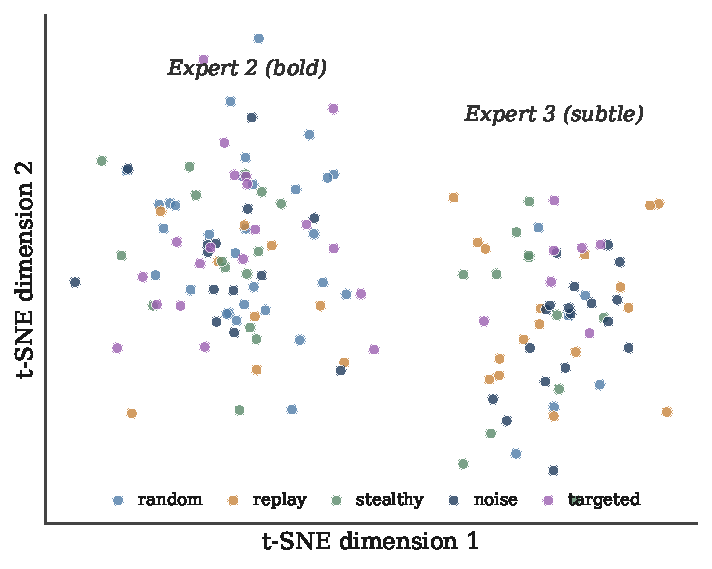
\includegraphics[width=0.85\textwidth]{figures/vocab_attackmoe}
  \caption{t-SNE projection of attacker perturbation vectors from
  the Attacker \moe{} on the Modena test set. Points are coloured
  by ground-truth attack type; marker shapes indicate which expert
  was selected by the router. The two active experts occupy
  non-overlapping regions of perturbation space.}
  \label{fig:vocab}
\end{figure}

\section{Implementation Details}
\label{sec:selfplay_implementation}

All experiments run on Apple-Silicon \textsc{mps} hardware (M-series
GPU). Training the pretrained Temporal \moe{} takes approximately
15 minutes per network. Self-play fine-tuning takes a further 15
minutes per network. Total compute for all experiments in this thesis
is under 4 hours on a single consumer laptop.

The full training configuration for the headline Modena self-play
run is:
\begin{itemize}
  \item Defender: pretrained Temporal \moe{},
    hidden dim 48, 6 experts, window 6.
  \item Attacker: \moe{} of 4 attackers,
    hidden dim 64, 2 GraphSAGE layers.
  \item $\varepsilon_p = 5.0$\,m, $k_p = 15$,
    $\varepsilon_q = 0.05$, $k_q = 10$.
  \item $\lambda_\text{recon} = 5.0$,
    $\lambda_\text{phys} = 0.05$,
    $\lambda_\text{div} = 0.5$,
    $\lambda_\text{bal} = 0.1$.
  \item Attacker steps $S_a = 3$, defender steps $S_d = 1$.
  \item Curriculum: $\tau = 0.85$, $\Delta\varepsilon = 0.5$,
    $\Delta k = 2$.
  \item Epochs: 60; best model by composite
    $(\mathrm{F1}_\text{anomaly} + \mathrm{F1}_\text{replay}) / 2$.
\end{itemize}
All code is available in \texttt{src/wdn/train\_selfplay.py} and the
flags are documented in the repository README.
